\documentclass{beamer}
\usetheme{manhattangoogle}  % Now it's a beamer presentation with the Manhattan College theme!

\usepackage{url}
\usepackage{graphicx}
\usepackage{fancyvrb}
\usepackage{MnSymbol, amsthm, amsfonts, amsmath, amssymb, amsxtra}
\usepackage{multirow}

\newcommand{\Z}{\mathbb{Z}}
\beamertemplatenavigationsymbolsempty

% Make a new command that will make a new subsection and a frame with the same title
\newcommand{\fst}[2]{\subsection{#1}\frame{\frametitle{#1} #2}}
\newcommand{\ft}[2]{\frame{\frametitle{#1} #2}}

% ~ instead of spaces prevents linebreaks
\title{People and Computers Agree on the Complexity of Small Art}
\author{Jonathan Langke and Peter Boothe}
\date{%

\includegraphics[height=.5in]{bridges-seoul-2014-logo-small.png}}
\institute[Manhattan College]{
\begin{tabular}{rl}%
    \url{jlangke22@gmail.com} & \multirow{3}{*}{
\includegraphics[height=.4in]{email_logo.png}}\\
    Computer Engineering '13 & \\
    Manhattan College & \\
    & \\
    \url{pboothe@gmail.com} & \multirow{3}{*}{
\includegraphics[height=.4in]{google.png}}\\
    (was) Computer Science @ Manhattan College & \\
    (now) Software Engineer @ Google & \\
\end{tabular}%
}

\begin{document}
\frame{\titlepage}
\section{What is art?}
\fst{This is art}{\begin{center}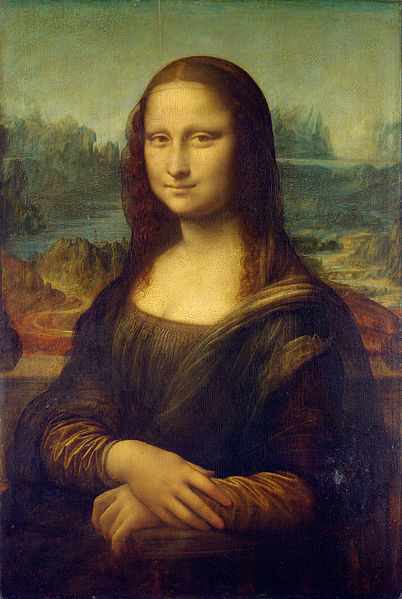
\includegraphics[height=2.5in]{monalisacolor.jpg}\\
\pause {\tt int $\times$ int $\to$ color}\end{center}}
\fst{Grayscale}{\begin{center}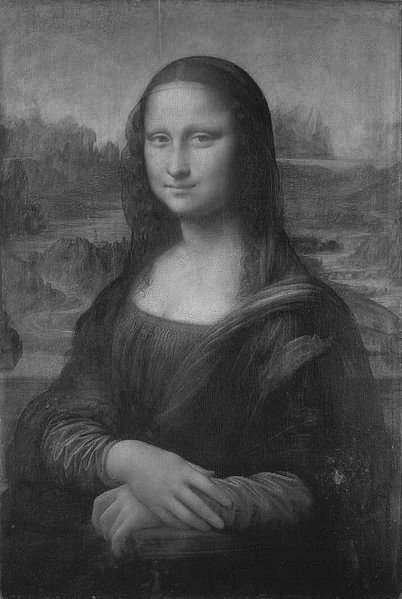
\includegraphics[height=2.5in]{monalisagray.jpg}\\
{\tt int $\times$ int $\to$ number}\end{center}}
\fst{Black and White}{\begin{center}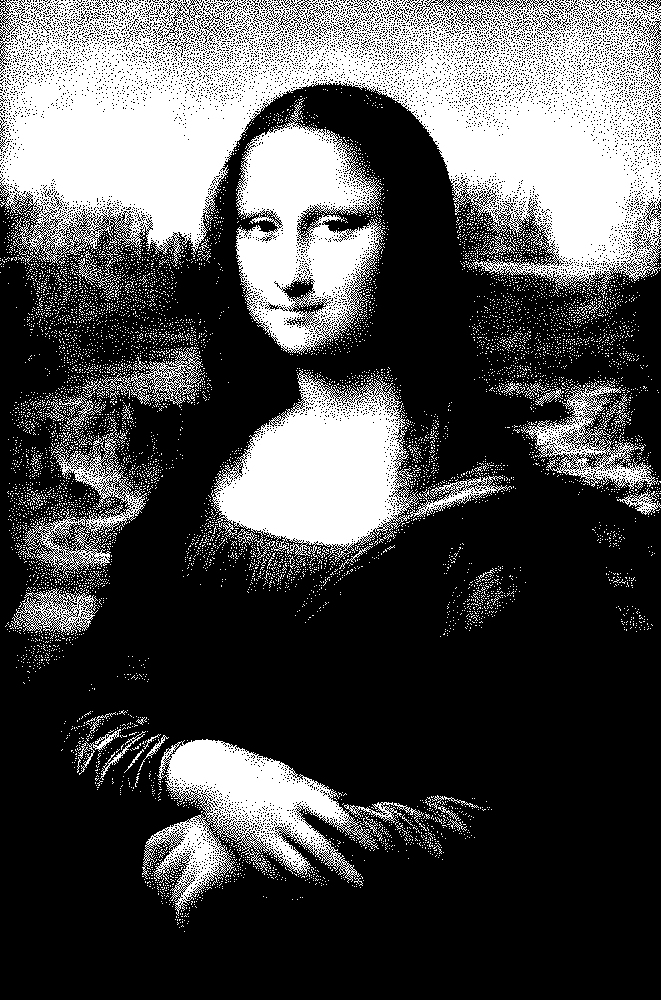
\includegraphics[height=2.5in]{../paper/monalisa_mono.jpg}\\
{\tt int $\times$ int $\to$ \{0, 1\}}\end{center}}
\ft{Black and White}{\begin{center}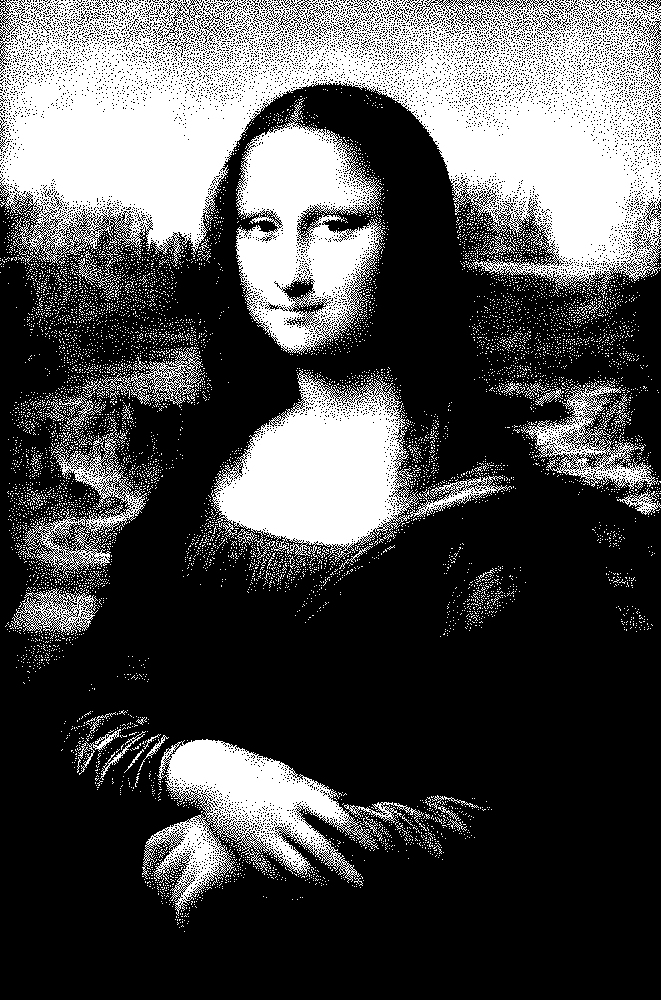
\includegraphics[height=2.5in]{../paper/monalisa_mono.jpg}\\
{\tt int $\times$ int $\to$ bool}\end{center}}
\ft{Black and White}{\begin{center}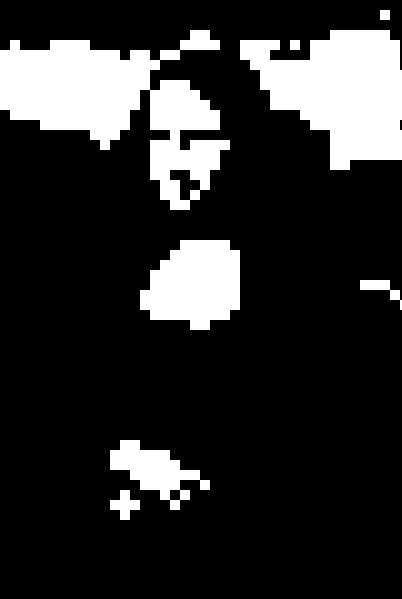
\includegraphics[height=2.5in]{monalisabwpixels.jpg}\\
{\tt int $\times$ int $\to$ bool}\end{center}}
\fst{Generalized}{\begin{center}Digital pictures are the output of evaluating a function at every pixel in the picture.\\
~\\
For black and white pictures, this function is of type:\\
~\\
{\LARGE \tt int $\times$ int $\to$ bool}\\
~\\
Human complexity has to do with the picture \\
Computer complexity has to do with the function
\end{center}}
\section{Computer complexity}
\fst{Kolmogorov Complexity}{
 {\LARGE The Kolmogorov complexity of an object is equal to the size of the smallest program that outputs that object.}

~\\
\pause All Turing-complete programming languages are equivalent\\
Provably impossible to calculate\\
Provably impossible to approximate
}
\fst{Formula complexity}{For us a ``formula'' is a well-typed fully-parenthesized expression built out of the atoms:
 \begin{center}{\tt \{ 0, 1, x, y, +, *, <, not, and, or, true, false \}}\end{center}
{\tt x} and {\tt y} are integer variables which hold the coordinates of the grid point.\\
~\\
{\LARGE The Formula complexity of an object is the size of the smallest formula whose output is that object.}\\
~\\
\pause Not Turing complete!\\
A matter of ``mere'' computation to calculate and enumerate!}
\fst{Computing formula complexity}{The algorithm to calculate the formula complexity of a picture is simple to describe: 

\begin{quote}
Enumerate all well-typed formulae in order of size. Stop when you have enumerated a formula whose output is the picture. The size of that formula is the formula complexity of the picture.
\end{quote}

\pause Horrendous runtime. Highly exponential. Do it anyway.\\
~\\
This terrible algorithm restricts the size of artworks we can consider.  In particular, we can only work with 9 pixel artworks --- 3 pixels by 3 pixels.  There are $2^9 = 512$ such artworks, but we will need to generate hundreds of billions of formulae.}
\section{All the art!}
\ft{}{
    \begin{center}
        
\includegraphics[width=3.5in]{alltheart.png}\\
        \url{http://hyperboleandahalf.blogspot.com/2010/06/this-is-why-ill-never-be-adult.html}
    \end{center}
}
\fst{All the 2x2 Art}{
\begin{tabular}{r c l}
Formula & FC & Picture \\
\tiny{none} & 0 & empty \\
\tiny{(true), (false)} & 1 &
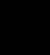
\includegraphics[width=.25in]{2x2/Shape1LVL1.png}~

\includegraphics[width=.25in]{2x2/Shape2LVL1.png} \\
\tiny{none} & 2 & empty \\
\tiny{(x $<$ 1), (y $<$ 1), (x $<$ y), (0 $<$ x), (0 $<$ y), (y $<$ x)} & 3 & 
\reflectbox{\rotatebox[origin=c]{180}{
\includegraphics[width=.25in]{2x2/Shape1LVL3.png}}}~
\reflectbox{\rotatebox[origin=c]{180}{
\includegraphics[width=.25in]{2x2/Shape2LVL3.png}}}~
\reflectbox{\rotatebox[origin=c]{180}{
\includegraphics[width=.25in]{2x2/Shape5LVL3.png}}}~
\reflectbox{\rotatebox[origin=c]{180}{
\includegraphics[width=.25in]{2x2/Shape6LVL3.png}}}~
\reflectbox{\rotatebox[origin=c]{180}{
\includegraphics[width=.25in]{2x2/Shape3LVL3.png}}}~
\reflectbox{\rotatebox[origin=c]{180}{
\includegraphics[width=.25in]{2x2/Shape4LVL3.png}}}\\
\tiny{(not (x $<$ y)), (not (y $<$ x))} & 4 & 
\reflectbox{\rotatebox[origin=c]{180}{
\includegraphics[width=.25in]{2x2/Shape2LVL4.png}}}~
\reflectbox{\rotatebox[origin=c]{180}{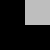
\includegraphics[width=.25in]{2x2/Shape1LVL4.png}}}\\
\tiny{((y + x) $<$ 1), ((y * x) $<$ 1), (0 $<$ (y + x)), (1 $<$ (y + x))} & 5 & 
\reflectbox{\rotatebox[origin=c]{180}{
\includegraphics[width=.25in]{2x2/Shape2LVL5.png}}}~
\reflectbox{\rotatebox[origin=c]{180}{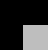
\includegraphics[width=.25in]{2x2/Shape1LVL5.png}}}~
\reflectbox{\rotatebox[origin=c]{180}{
\includegraphics[width=.25in]{2x2/Shape3LVL5.png}}}~
\reflectbox{\rotatebox[origin=c]{180}{
\includegraphics[width=.25in]{2x2/Shape4LVL5.png}}}\\
\tiny{none} & 6 & empty \\
\tiny{((y $<$ x) or (x $<$ y))} & 7 &
\reflectbox{\rotatebox[origin=c]{180}{
\includegraphics[width=.25in]{2x2/Shape1LVL7.png}}}\\
\tiny{(not ((y $<$ x) or (x $<$ y)))} & 8 &
\reflectbox{\rotatebox[origin=c]{180}{
\includegraphics[width=.25in]{2x2/Shape1LVL8.png}}}
\end{tabular}
}

\fst{Selected 3x3 art}{
\begin{tabular}{r c l}
Formula & FC & Picture \\
\small{(x $<$ y)} & 3 & \reflectbox{
\includegraphics[width=.85in]{../paper/3x3pics/311.png}} \\ % Different bitpattern because we want black=true
\small{((not (y $<$ (x * y))) and ((y * y) $<$ (x + (y + y))))} & 16 & \reflectbox{
\includegraphics[width=.85in]{../paper/3x3pics/353.png}} % Different bitpattern because we want black=true
\end{tabular}
}

\fst{All the 3x3 art}{
    \begin{center}
        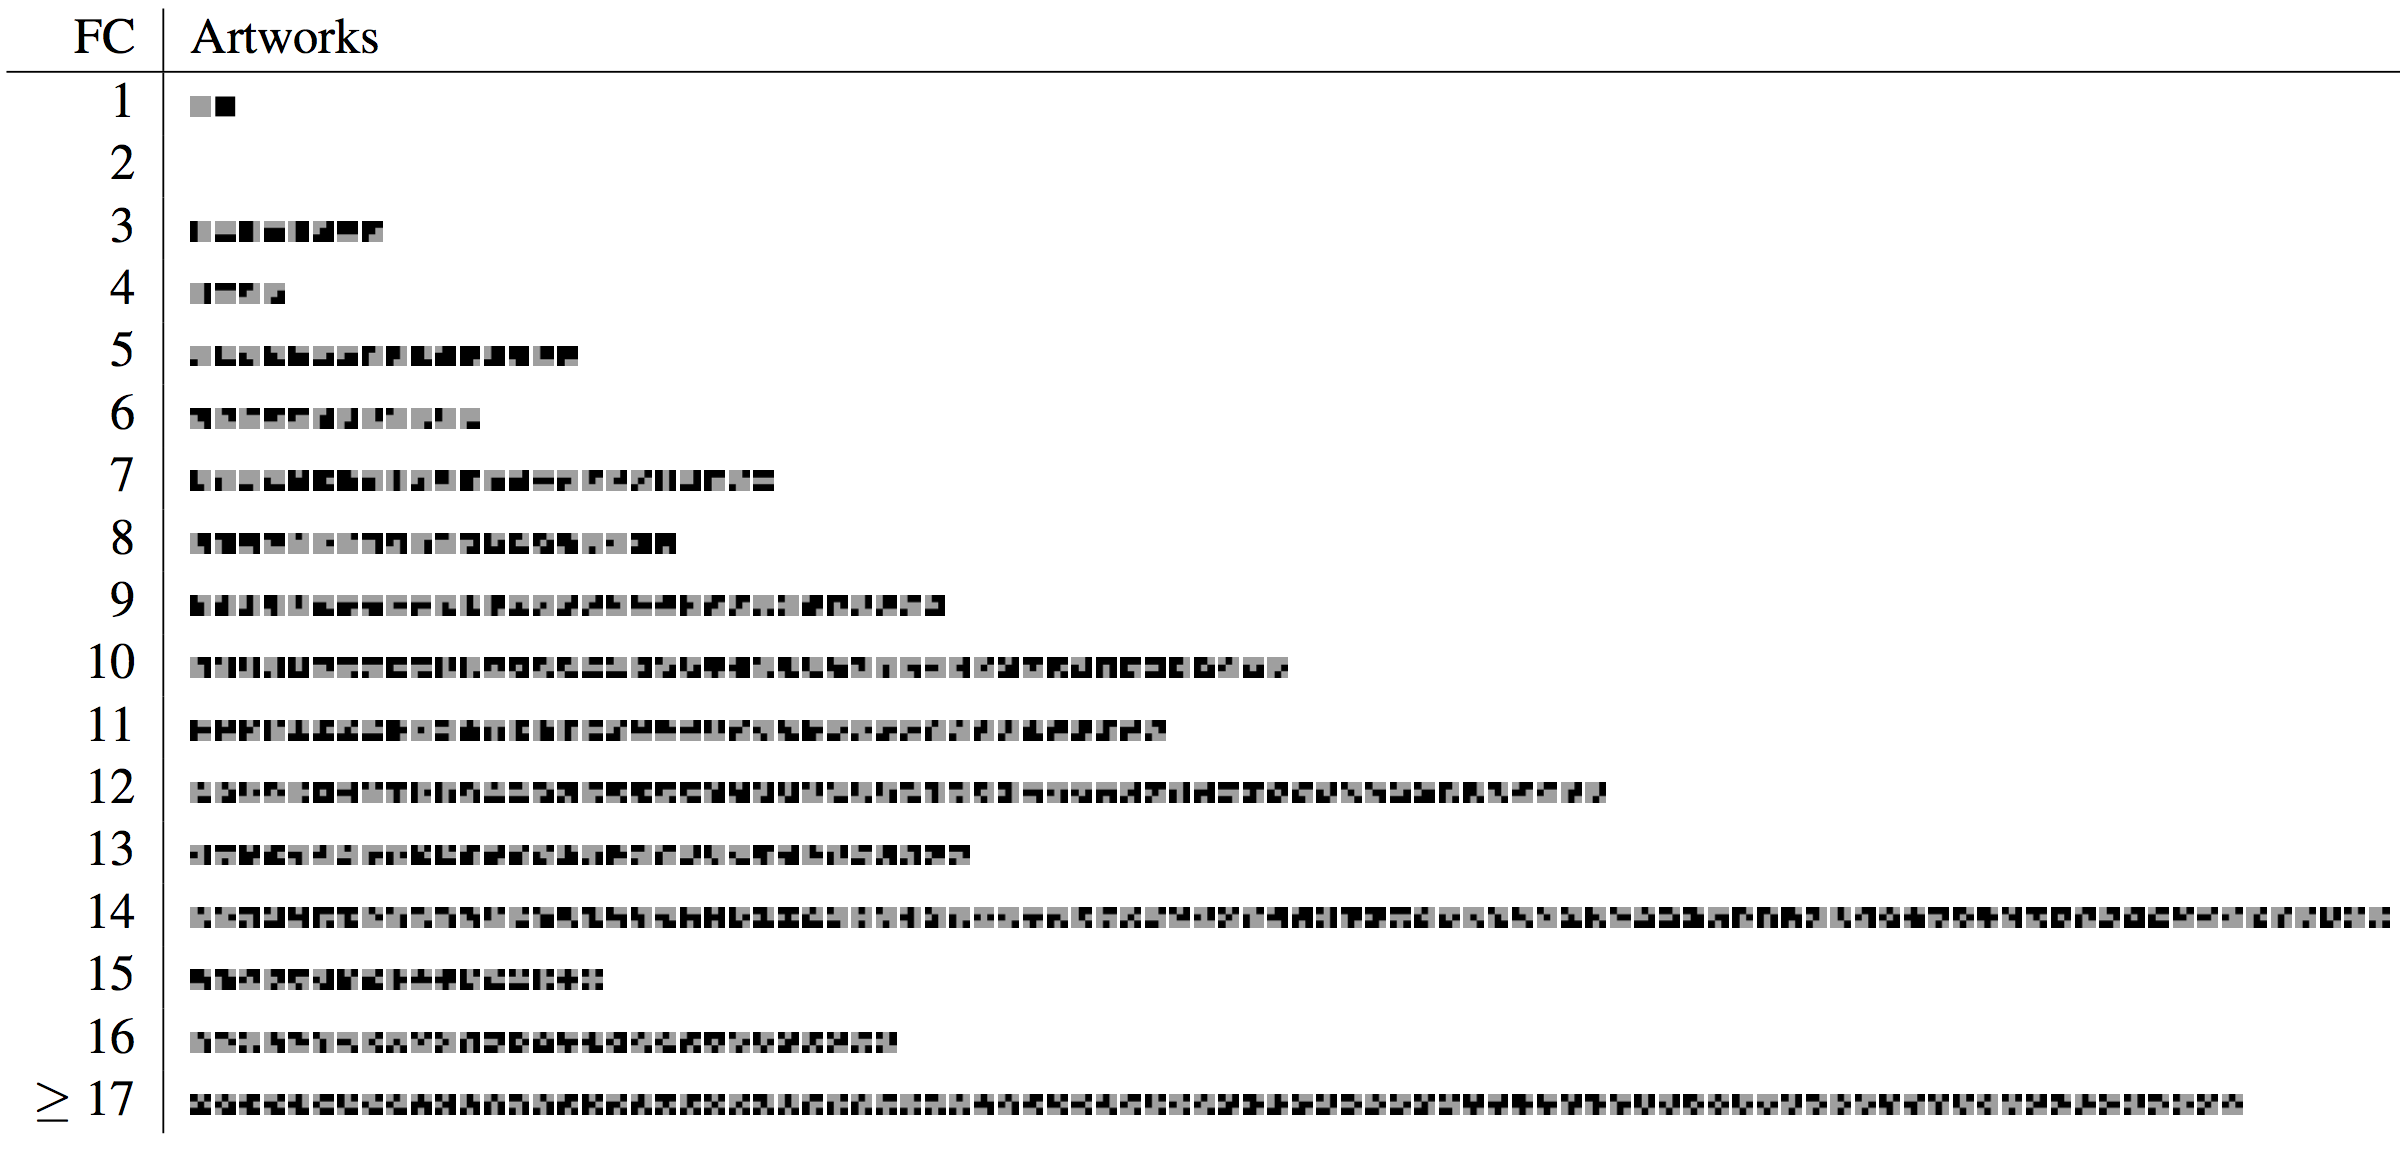
\includegraphics[width=4.5in]{all3x3.png}
    \end{center}
}
\subsection{Zooming in}
\ft{}{
\vspace{-.1in}
    \begin{center}
        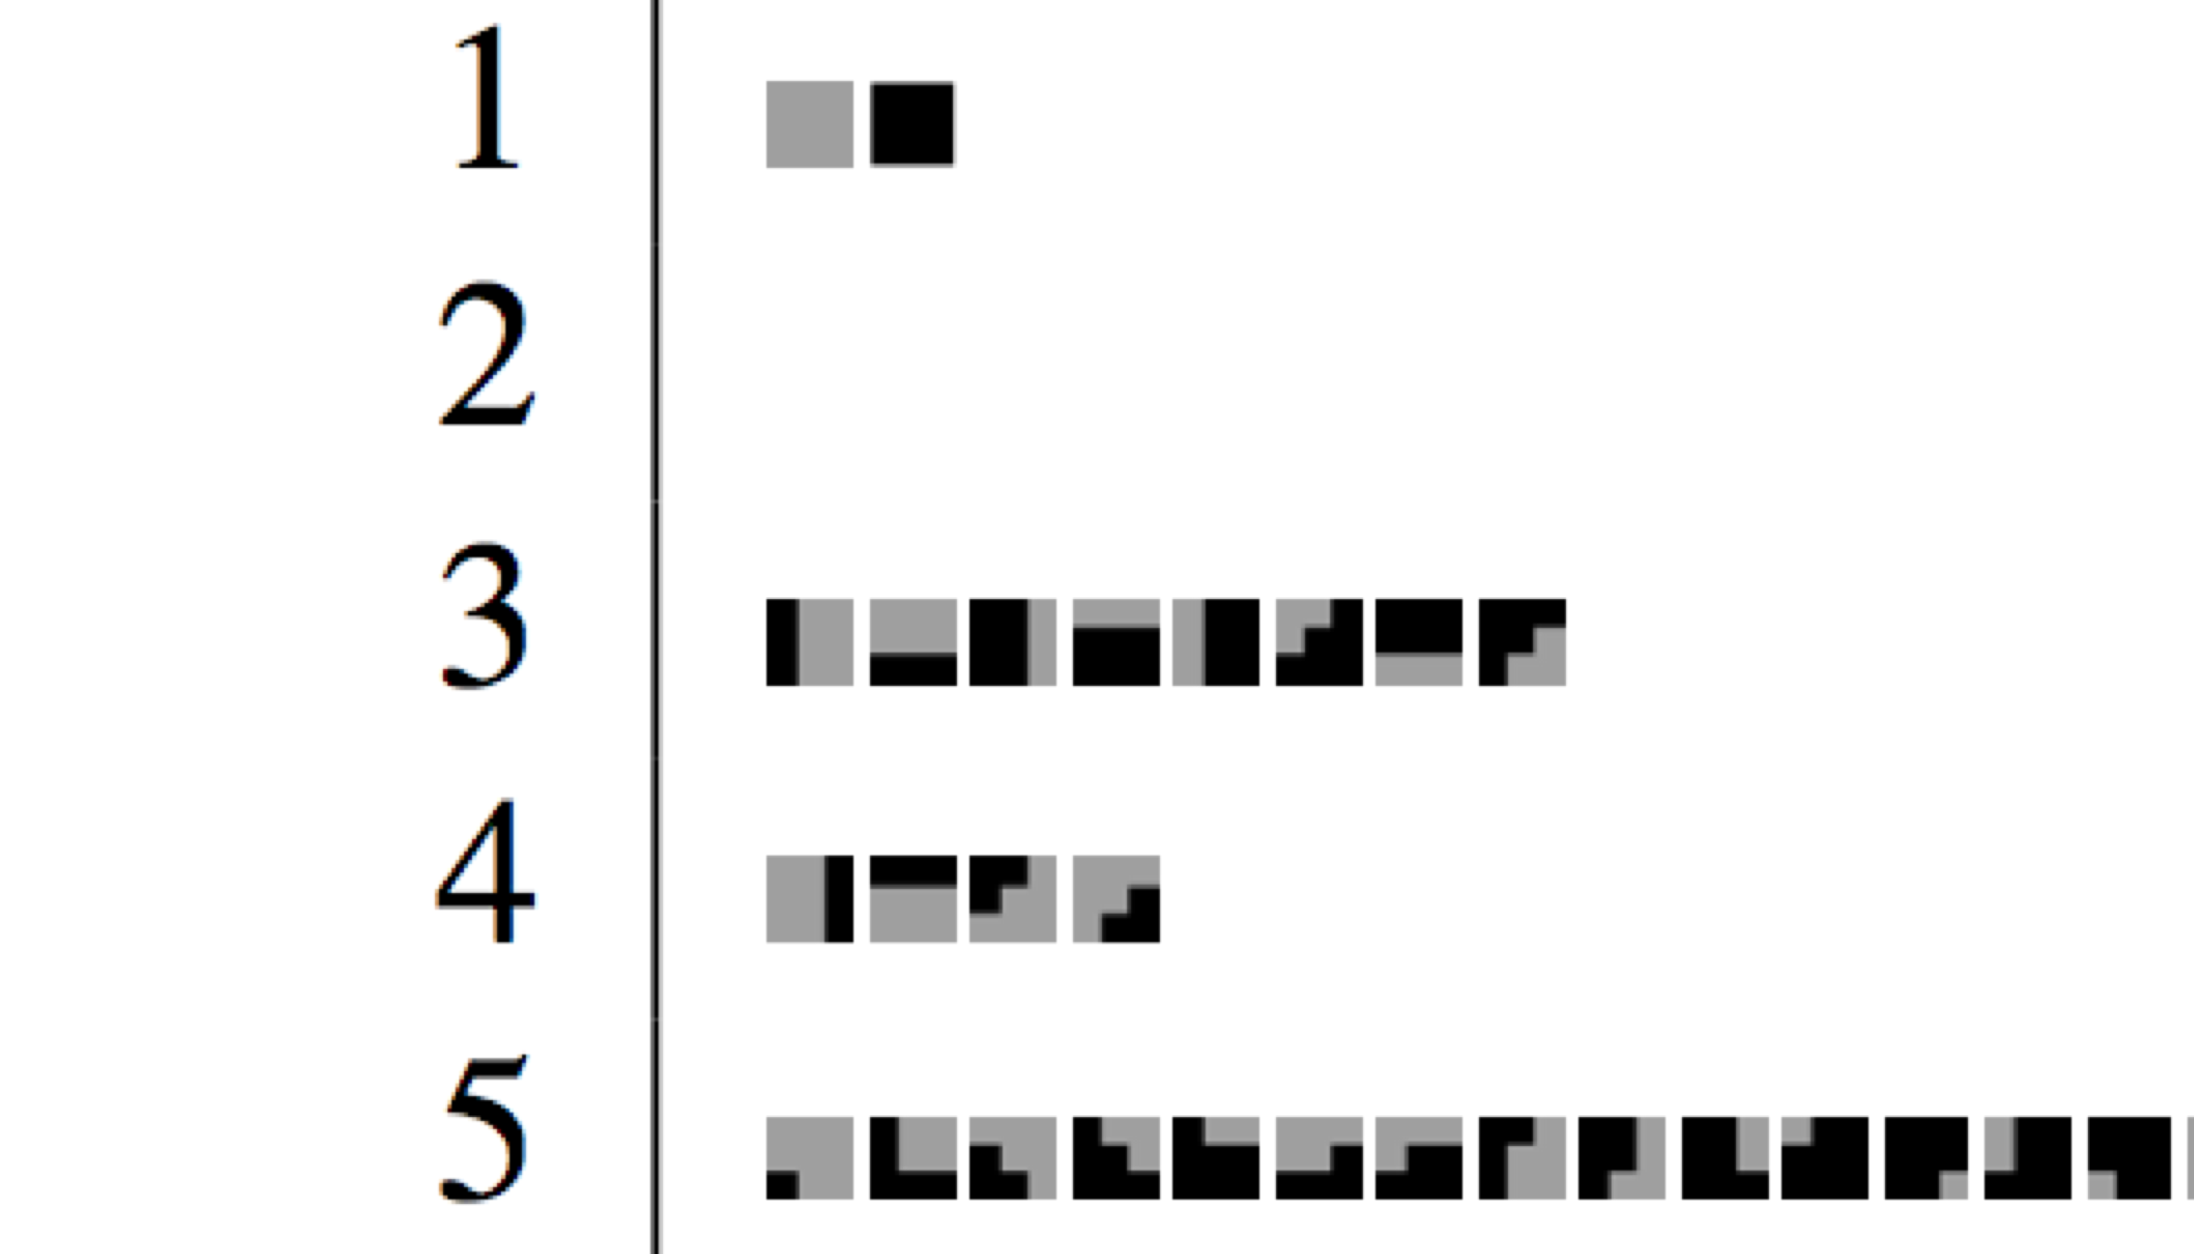
\includegraphics[width=4.5in]{3x3top.png}
    \end{center}
}
\ft{}{
\vspace{-.2in}
    \begin{center}
        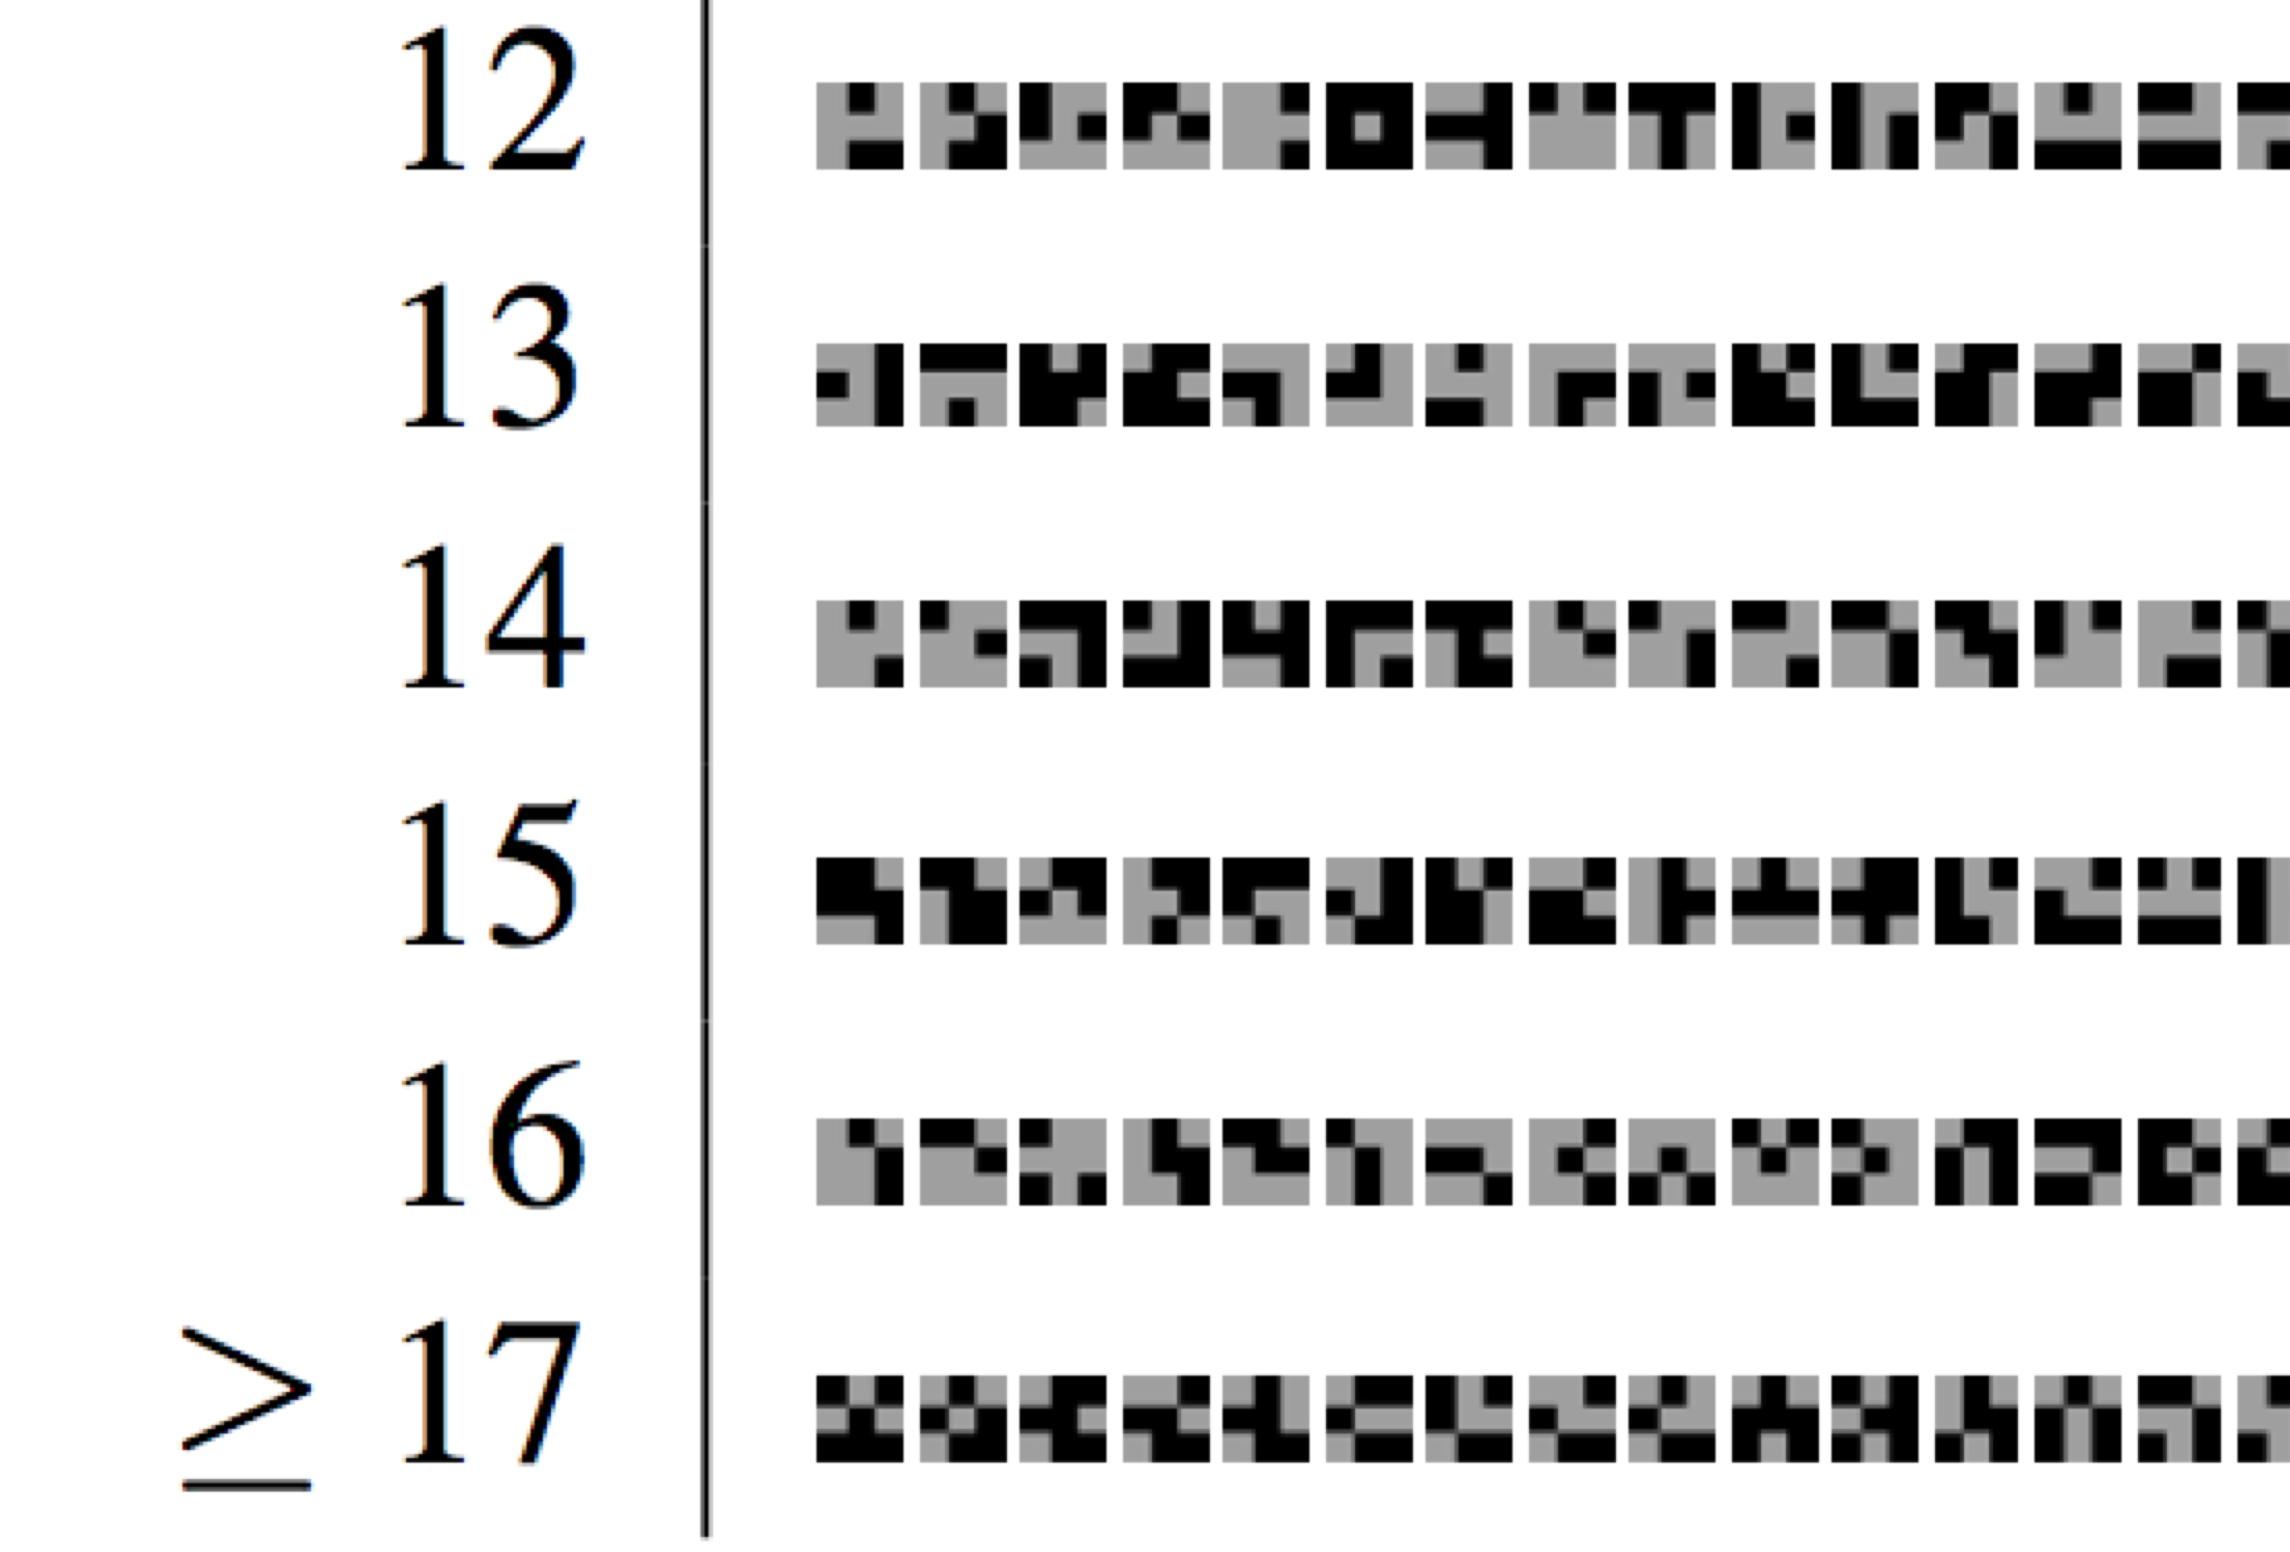
\includegraphics[width=4.5in]{3x3bottom.png}
    \end{center}
}

\section{Human complexity}
\fst{Visual complexity is hard to measure}{
\begin{itemize}
\item Intuitive. 
\item Complex. 
\item ``I know it when I see it.'' 
\item Hard to explain.
\end{itemize}

\pause
\begin{itemize}
\item Can't be measured absolutely.
\item Can be measured relatively!
\end{itemize}
}

\fst{Our survey}{
    \begin{center}
        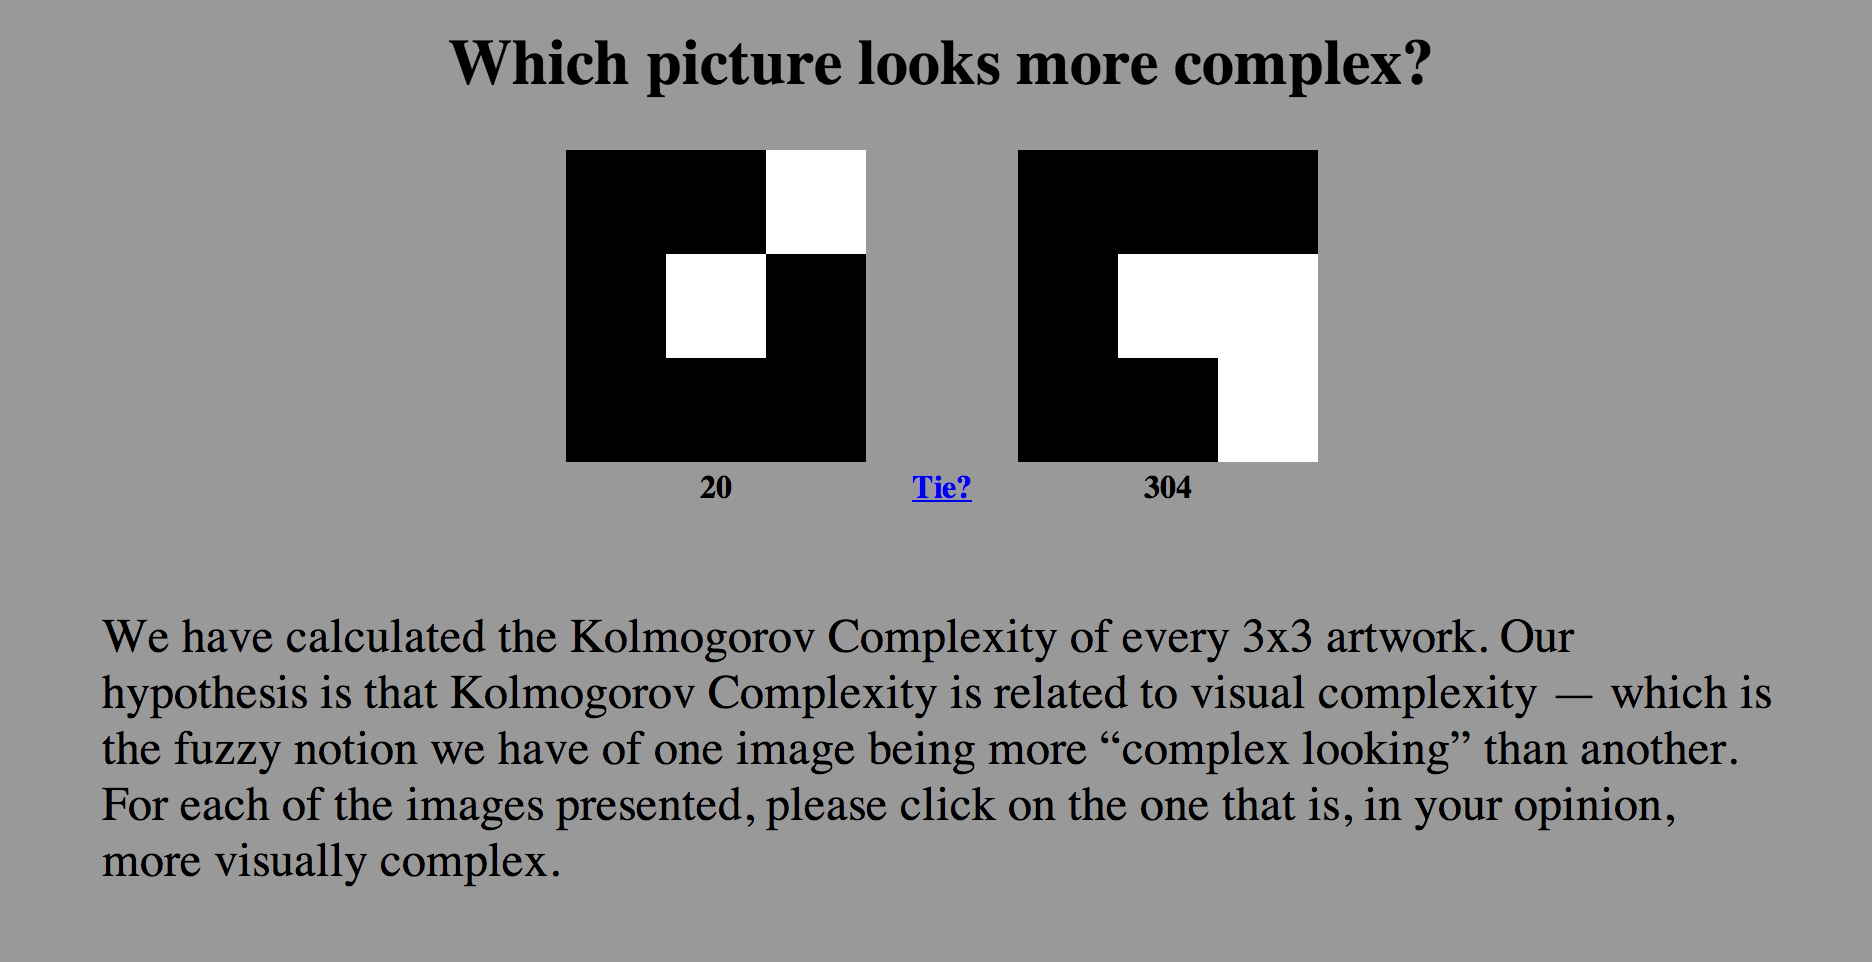
\includegraphics[width=4.5in]{survey.png}
    \end{center}
}

\fst{Measure like chess}{
\begin{itemize}
\item Perform repeated pairwise comparisons, asking test subjects ``Which of these is more visually complex?''
\item Treat each comparison as a match with a winner and a loser.  
\item Use the TrueSkill algorithm to assign a strength rating to each artwork based on match results.

\pause 
\item Passed it around among undergrads and Twitter, got many thousands of comparisons.
\end{itemize}
}

\section{Results}

\fst{It correlates!}{
\vspace{-.25in}
    \begin{center}
        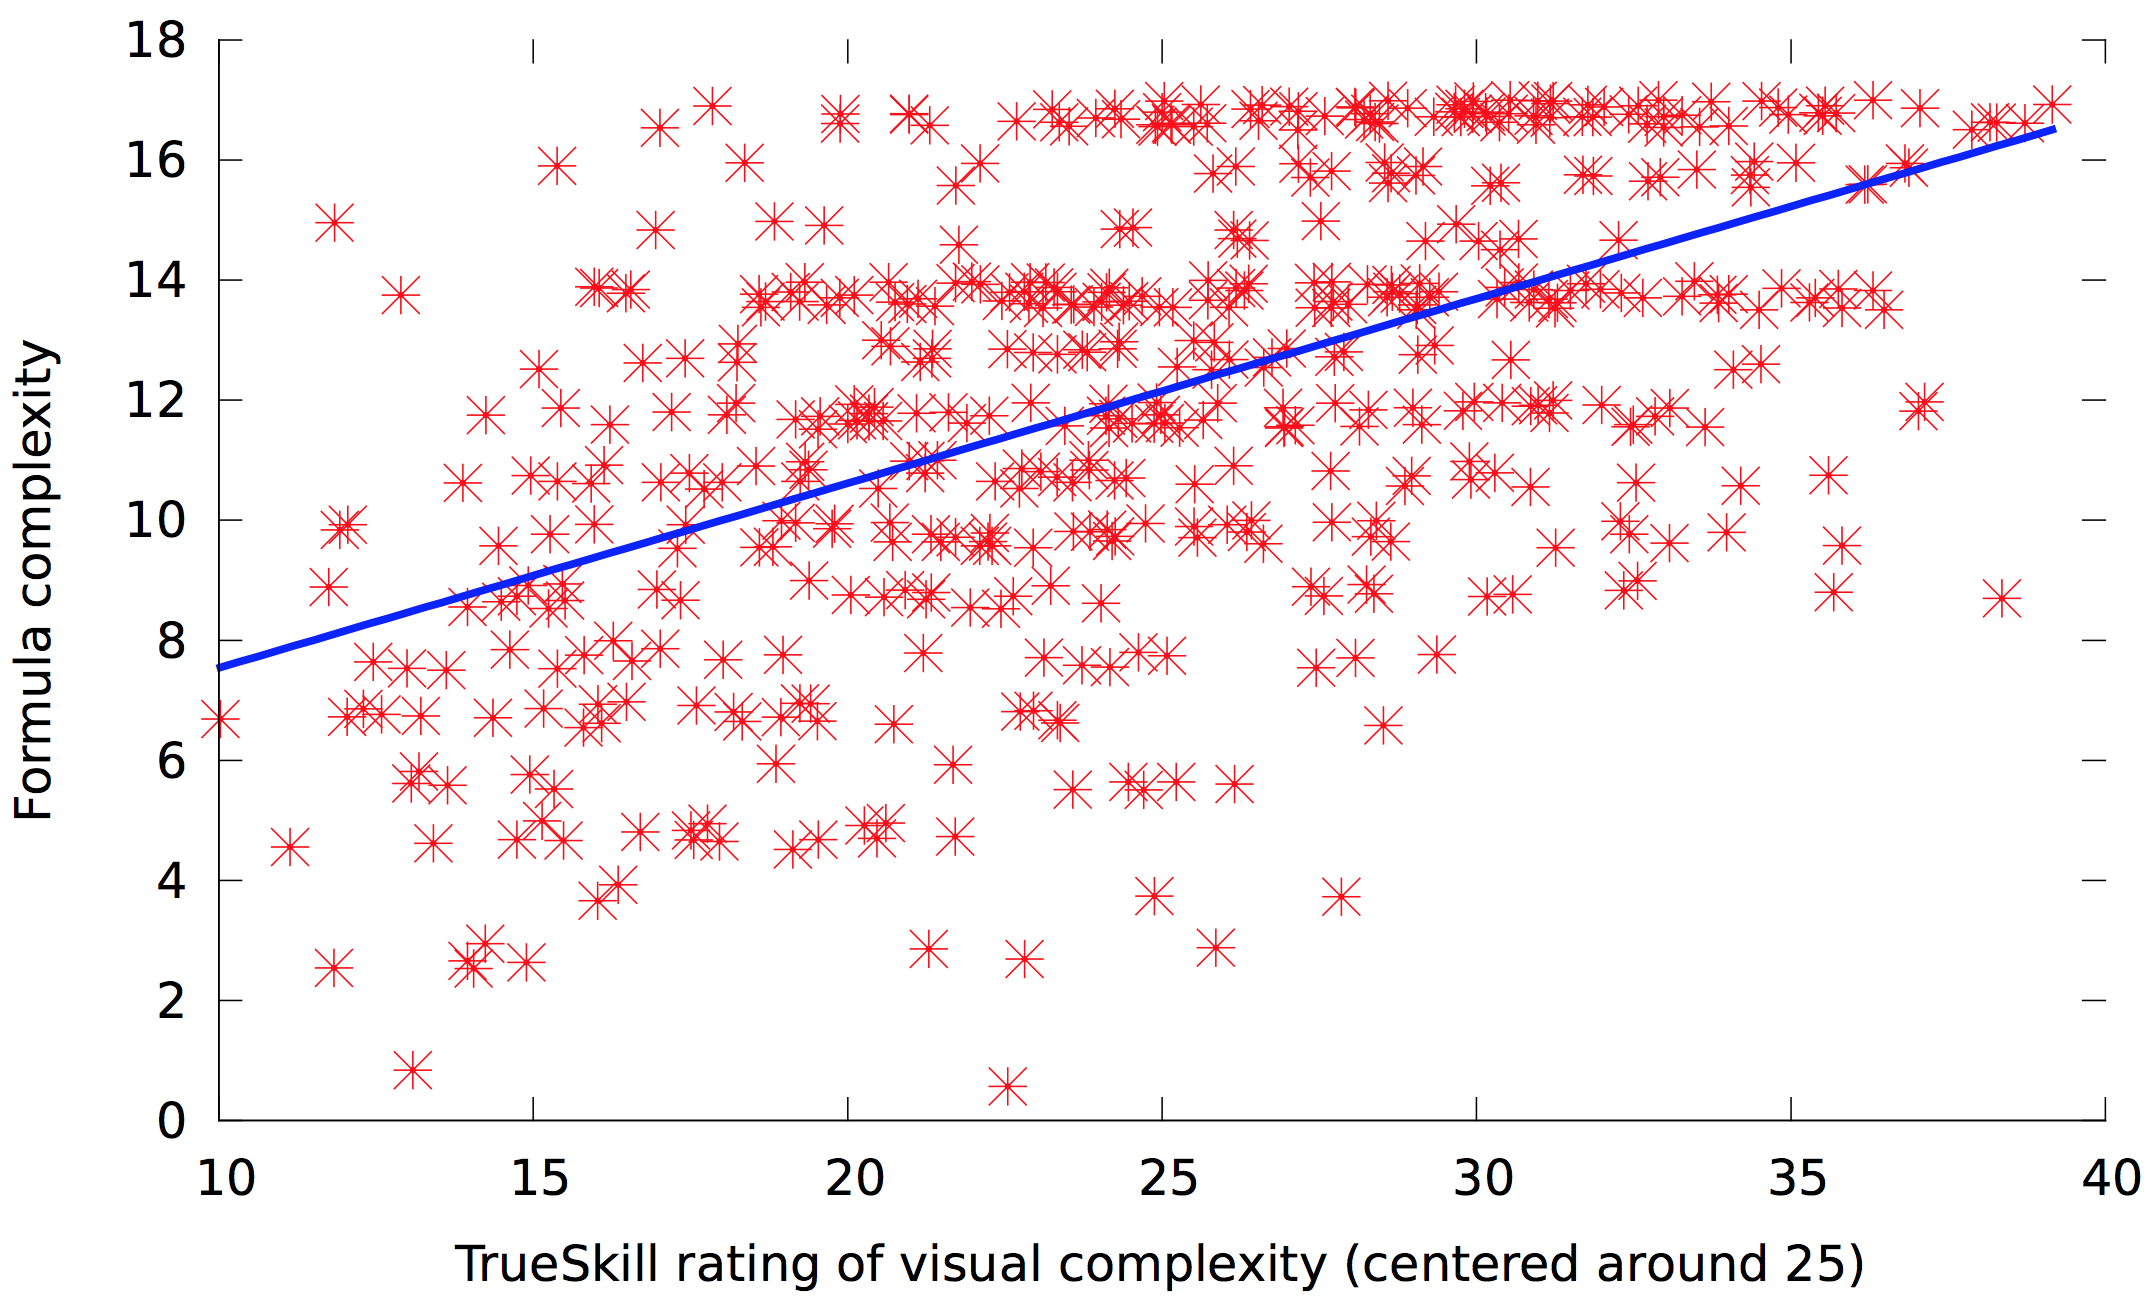
\includegraphics[width=4.5in]{correlate.png}
    \end{center}
}

\subsection{Small changes}

\ft{One-pixel differences}{
\vspace{-.25in}
    \begin{center}
        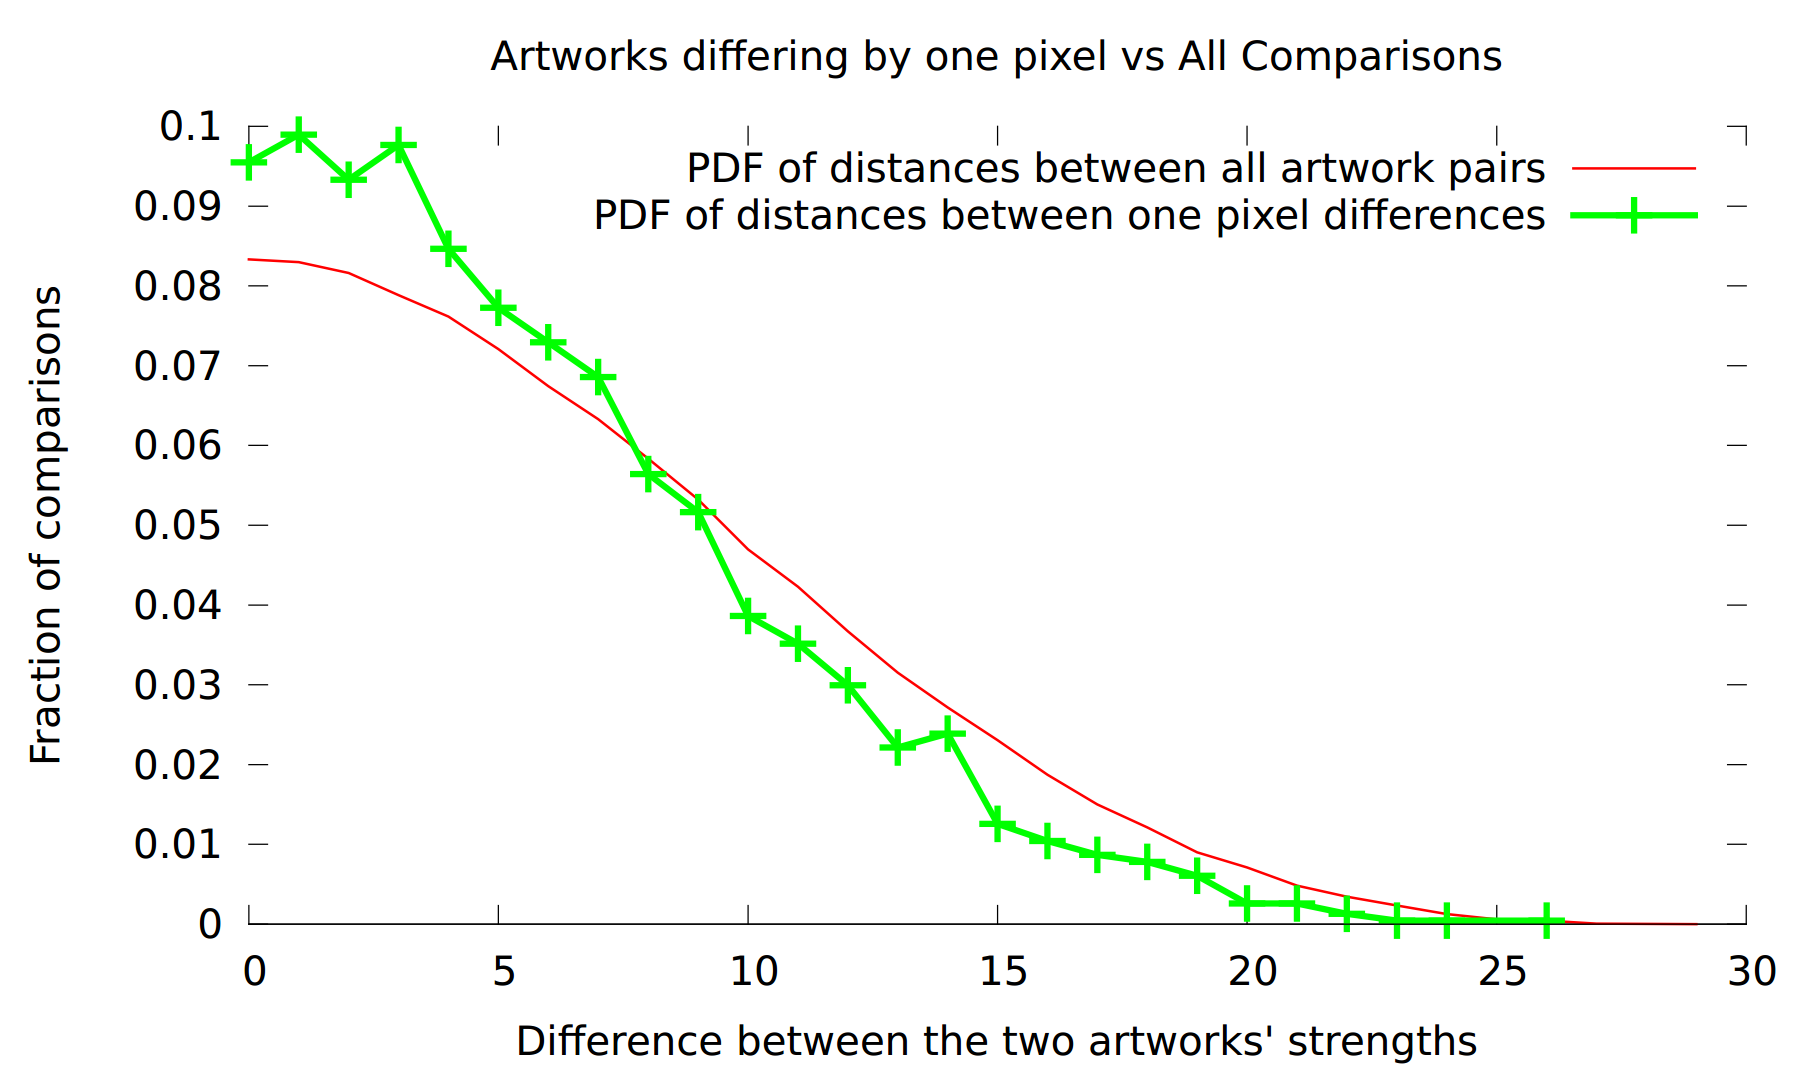
\includegraphics[width=4.5in]{onepixel.png}
    \end{center}
}

\ft{Swap x and y}{
\vspace{-.25in}
    \begin{center}
        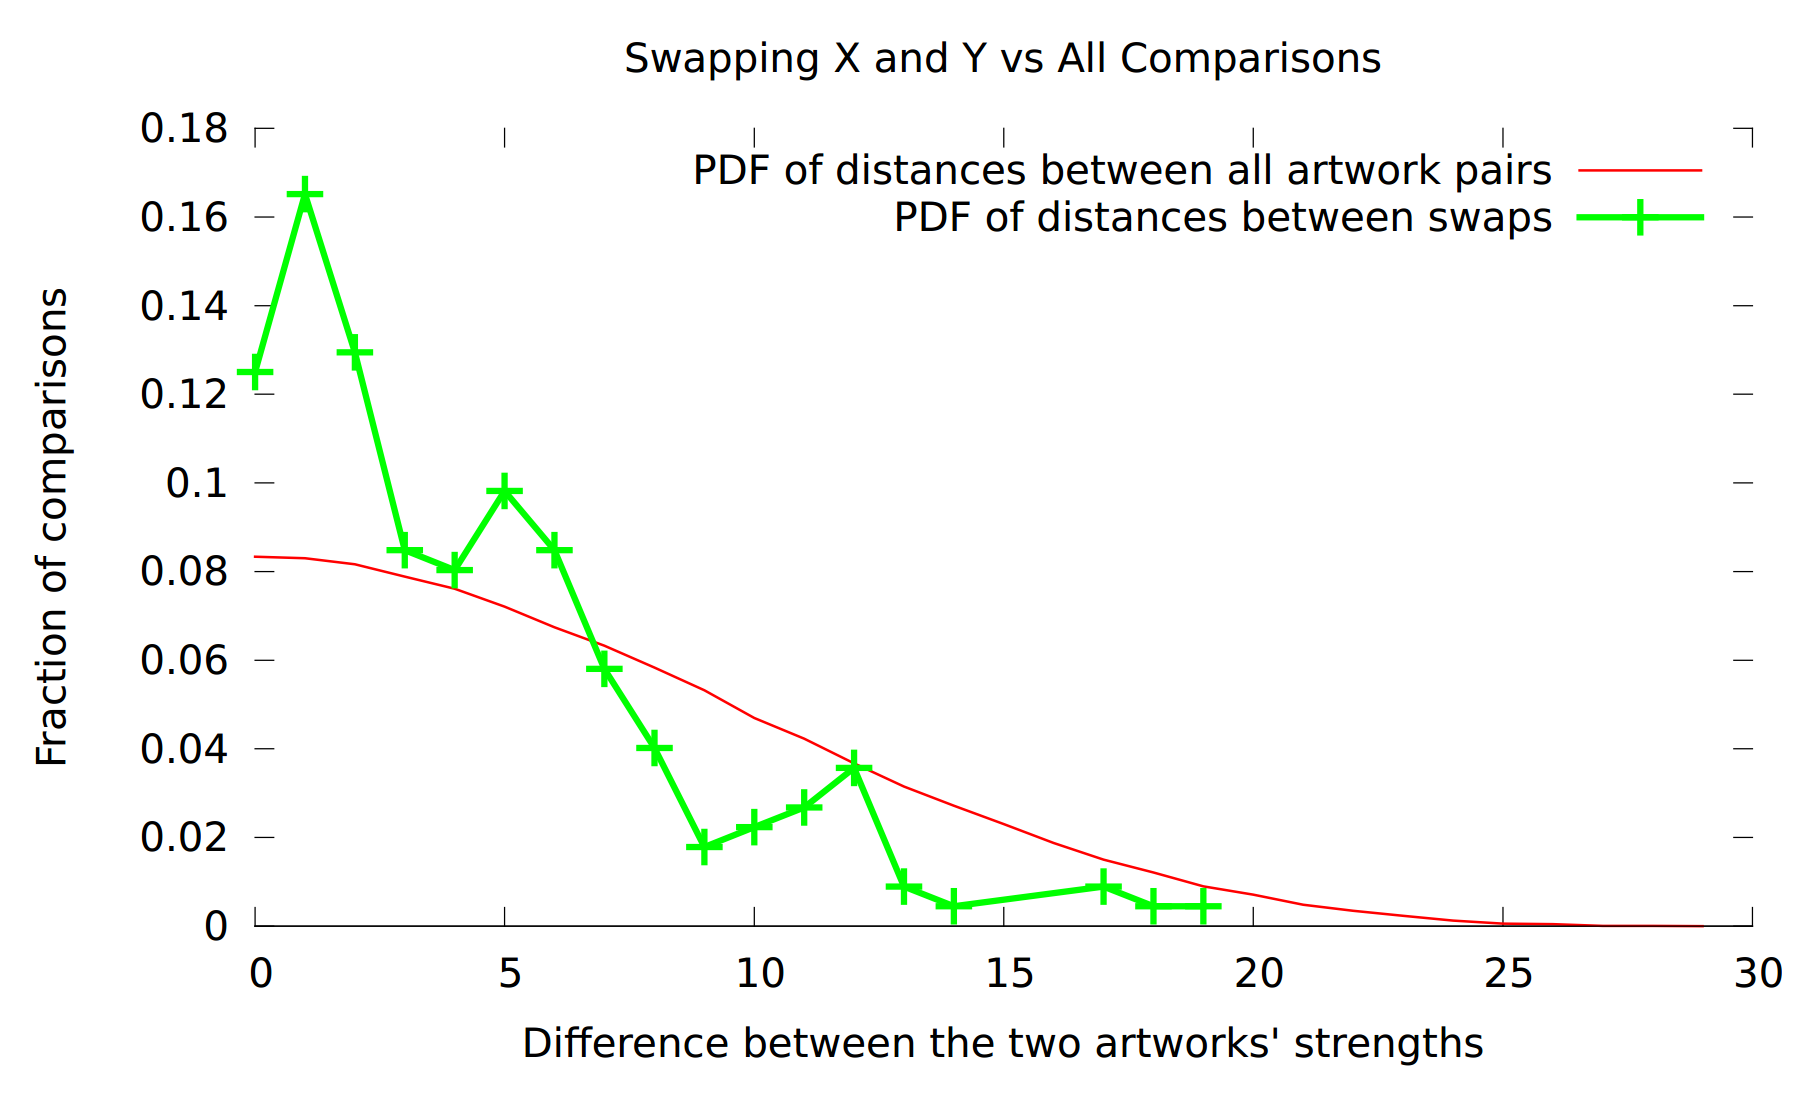
\includegraphics[width=4.5in]{diagonal.png}
    \end{center}
}

\ft{Swap black and white}{
\vspace{-.25in}
    \begin{center}
        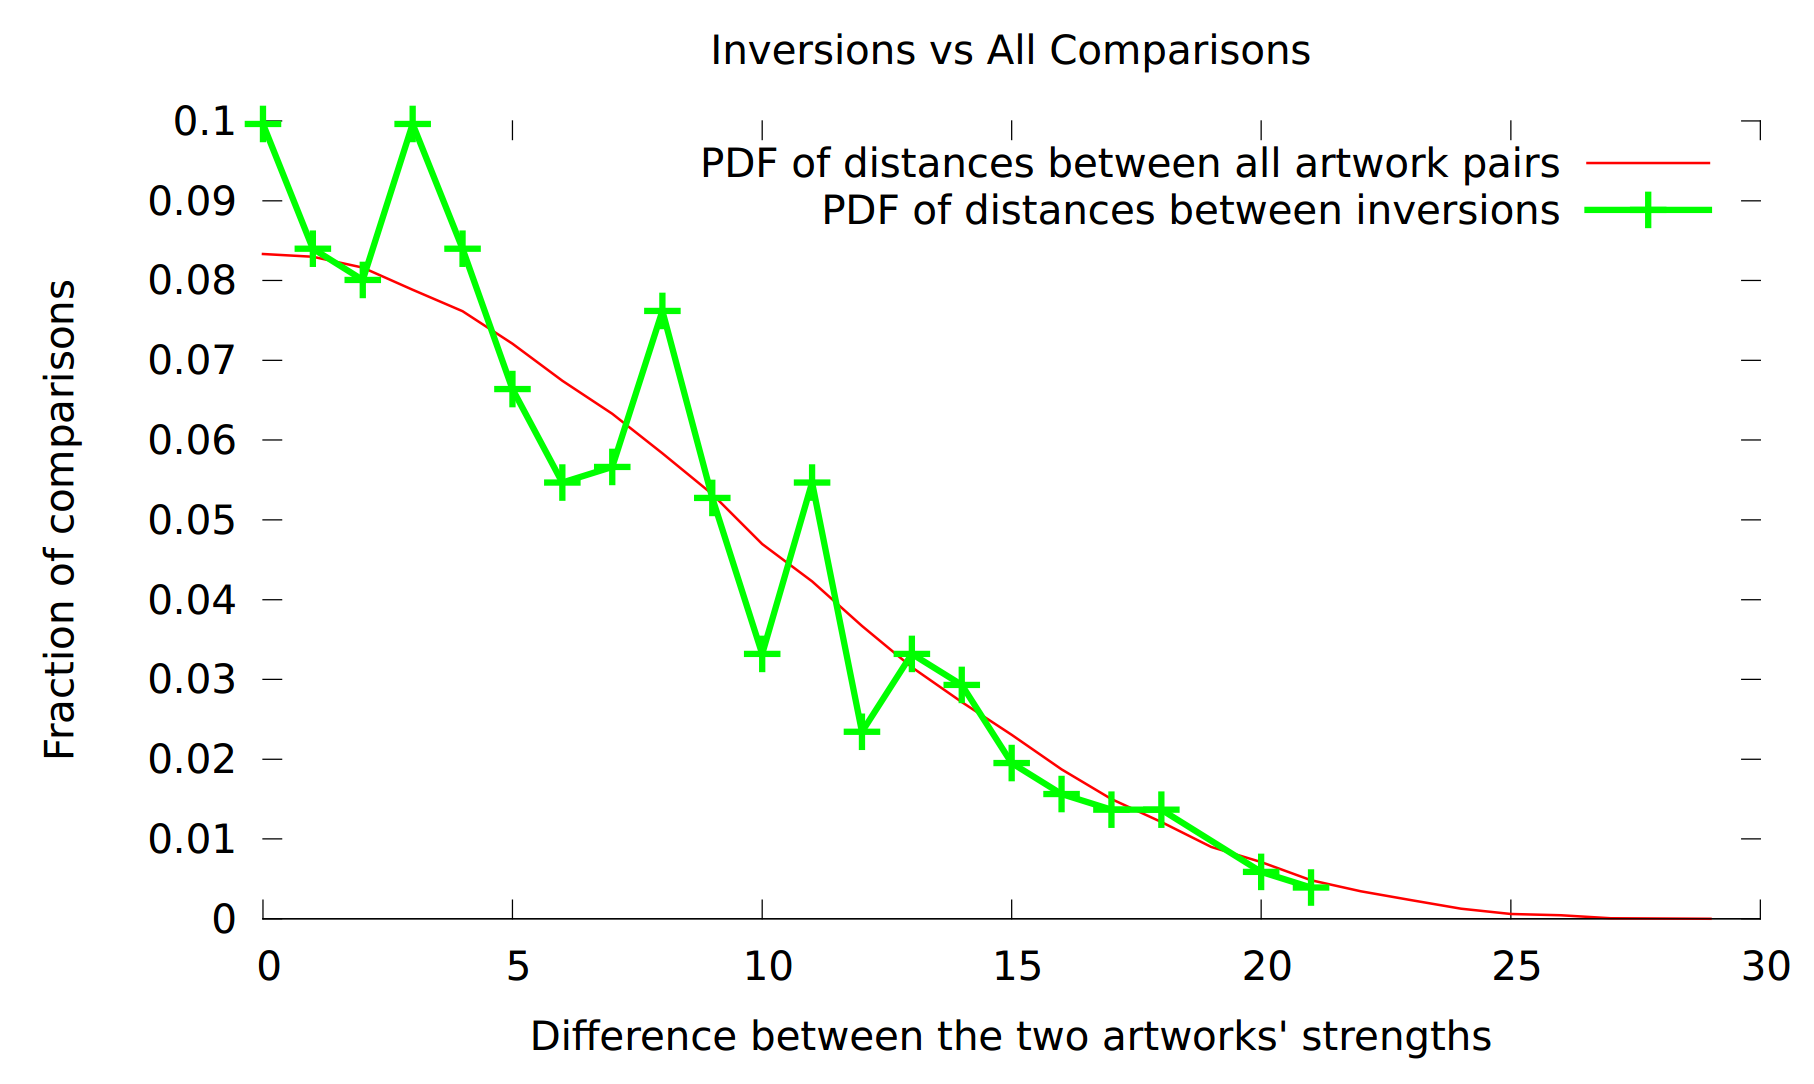
\includegraphics[width=4.5in]{invert.png}
    \end{center}
}

\fst{Threats to validity}{
\begin{itemize}
\item We only surveyed WEIRD\footnote{Western, educated, industrialized, rich, democratic} CS people. 
\item The missing data of the $\ge17$ artworks
\item The art was tiny
\end{itemize}
}

\fst{Future work}{
\begin{itemize}
\item Wait for computers to get faster, re-run the generation process to find the missing data.
\item Try using Levin Complexity instead of formula complexity or Kolmogorov complexity.
\item What atoms make for a formula complexity that best matches people's visual complexity?
\end{itemize}
}

\fst{Summary}{
\vspace{-.2in}

We have:
\begin{enumerate}
    \item \ldots established a mapping between functions and art
    \item \ldots defined ``formula complexity'', a low-power version of KC
    \item \ldots found the formula complexity of almost all 3x3 artworks
    \item \ldots asked people to compare the visual complexity of these artworks
    \item \ldots generated a TrueSkill rating for the visual complexity of each artwork
    \item \ldots found that the two measures correlate!
\end{enumerate}

\begin{center}
\pause {\LARGE People and computers agree on the complexity of small art!}

\pause ~\\ 
{\Large Questions?}
\end{center}
}
\end{document}
